%%%%%%%%%%%%%%%%%%%%%%%%%%%%%%%%%%%%%%%%%%%%%%%%%%%%%%%%%%%%%%%%%%
% Sample template for MIT Junior Lab Student Written Summaries
% Available from https://urldefense.proofpoint.com/v2/url?u=http-3A__web.mit.edu_8.13_www_Samplepaper_sample-2Dpaper.tex&d=DwICAg&c=sJ6xIWYx-zLMB3EPkvcnVg&r=D88uS55Tats-jlFQAC1XryFUYq8B7Lk3StFbXzgsiB4&m=ohtd7ngjfrVvxFRQ914sbsc86_Im41uKSVc3O_ix3gM&s=-m6lcQoQ6TleIzATgu7ICUGL_8_Tjk_wISjMqVPHw8s&e= 
%
%  Edited by Aykut C. Satici on July 2022.
%  Edited by Aykut C. Satici on February 2022.
%  Edited by T Saab July 2021.
%  Last Updated April 12, 2007
%
% Adapted from the American Physical Societies REVTeK-4 Pages
% at https://urldefense.proofpoint.com/v2/url?u=http-3A__publish.aps.org&d=DwICAg&c=sJ6xIWYx-zLMB3EPkvcnVg&r=D88uS55Tats-jlFQAC1XryFUYq8B7Lk3StFbXzgsiB4&m=ohtd7ngjfrVvxFRQ914sbsc86_Im41uKSVc3O_ix3gM&s=0MkBr6VsOTYVW97Jm2x26uabjoQ1HT5VVAQ0au7898g&e= 
%
% ADVICE TO STUDENTS: Each time you write a paper, start with this
%    template and save under a new filename.  If convenient, don't
%    erase unneeded lines, just comment them out.  Often, they
%    will be useful containers for information.
%
%%%%%%%%%%%%%%%%%%%%%%%%%%%%%%%%%%%%%%%%%%%%%%%%%%%%%%%%%%%%%%%%%%


%%%%%%%%%%%%%%%%%%%%%%%%%%%%%%%%%%%%%%%%%%%%%%%%%%%%%%%%%%%%%%%%%%
% PREAMBLE
% The preamble of a LaTeX document is the set of commands that precede
% the \begin{document} line.  It contains a \documentclass line
% to load the REVTeX-4 macro definitions and various \usepackage
% lines to load other macro packages.
%
% ADVICE TO STUDENTS: This preamble contains a suggested set of
%     class options to generate a ``Junior Lab'' look and feel that
%     facilitate quick review and feedback from one's peers, TA's
%     and section instructors.  Don't make substantial changes without
%     first consulting your section instructor.
%%%%%%%%%%%%%%%%%%%%%%%%%%%%%%%%%%%%%%%%%%%%%%%%%%%%%%%%%%%%%%%%%%

\documentclass[aps,twocolumn,twoside,secnumarabic,balancelastpage,amsmath,amssymb,nofootinbib]{revtex4}

% Documentclass Options
    % aps, prl, rmp stand for American Physical Society, Physical Review Letters, and Reviews of Modern Physics, respectively
    % twocolumn permits two columns, of course
    % nobalancelastpage doesn't attempt to equalize the lengths of the two columns on the last page
        % as might be desired in a journal where articles follow one another closely
    % amsmath and amssymb are necessary for the subequations environment among others
    % secnumarabic identifies sections by number to aid electronic review and commentary.
    % nofootinbib forces footnotes to occur on the page where they are first referenced
        % and not in the bibliography
    % REVTeX 4 is a set of macro packages designed to be used with LaTeX 2e.
        % REVTeX is well-suited for preparing manuscripts for submission to APS journals.

%\usepackage{lgrind}        % convert program listings to a form includable in a LaTeX document
% \usepackage[export]{adjustbox}
\usepackage{amsmath}
\usepackage{amssymb}
\usepackage{amsthm}
\usepackage{xcolor}
\usepackage{caption}
\captionsetup[figure]{font=small}
\usepackage{chapterbib}    % allows a bibliography for each chapter (each labguide has it's own)
\usepackage{enumitem}
\usepackage{epsfig}
\usepackage{epstopdf}
% \usepackage[top=1in, bottom=1in, left=1in, right=1in]{geometry}
\usepackage{graphics}      % standard graphics specifications
\usepackage[]{graphicx}      % alternative graphics specifications
\graphicspath{ {./figures/} }
\usepackage{lipsum}
% \usepackage{longtable}     % helps with long table options
\usepackage{mathrsfs}
% \usepackage{multicol}
\usepackage{multirow}
\usepackage{nicefrac}
% \usepackage{bm}            % special 'bold-math' package
\usepackage{scalerel}
\usepackage{subcaption}
\usepackage{tabularx}
% \usepackage{titlesec}
\usepackage{url}
\usepackage{xfrac}
\usepackage{verbatim}			% for comment environment
%\usepackage{asymptote}     % For typesetting of mathematical illustrations
%\usepackage{thumbpdf}
\usepackage[colorlinks=true]{hyperref}  % this package should be added after all others
\hypersetup{
pdftitle={Project Report Template},
linkbordercolor=orange,
citebordercolor=blue,
% pdfborder={0 0 1},
urlbordercolor=blue
}
\usepackage[textsize=footnotesize]{todonotes}
\usepackage{tikz}
\usetikzlibrary{graphs,quotes,arrows,patterns,decorations.pathmorphing}

%Next line moves text up a bit without changing text area size  
\addtolength\topmargin{-.5\topmargin} %increases the top margin by half.



\makeatletter
\newcommand{\rmnum}[1]{\romannumeral #1}
\newcommand{\Rmnum}[1]{\expandafter\@slowromancap\romannumeral #1@}
\makeatother


\newcommand{\bmat}[1]{\begin{bmatrix}#1\end{bmatrix}}
\newcommand{\ubar}[1]{\text{\b{$#1$}}}
\newcommand{\norm}[2]{\|{#1}\|_{{}_{#2}}}
\newcommand{\abs}[1]{\left|{#1}\right|}

\newcommand{\mbf}[1]{\mathbf{#1}}
\newcommand{\mc}[1]{\mathcal{#1}}
\newcommand{\dd}{\operatorname{d}\!}
\newcommand{\muc}[2]{\multicolumn{#1}{c}{#2}}
\newcommand*\Eval[3]{\left.#1\right\rvert_{#2}^{#3}}
\newcommand{\inner}[1]{\left\langle#1\right\rangle}
\newcommand{\pd}[2]{\frac{\partial #1}{\partial #2}}
\newcommand{\pdd}[2]{\frac{\partial^2 #1}{\partial #2^2}}
\newcommand{\vectornorm}[1]{\left|\left|#1\right|\right|}
\newcommand\sbullet[1][.5]{\mathbin{\vcenter{\hbox{\scalebox{#1}{$\bullet$}}}}}

\newtheorem{defn}{Definition}
\newtheorem*{thm*}{Theorem}
\newtheorem{thm}{Theorem}[section]
\newtheorem{lem}[thm]{Lemma}
\newtheorem{prop}{Proposition}[section]
\newtheorem{rem}{Remark}
% \newtheorem*{lem2}{Lemma}
% \newtheorem*{prop2}{Proposition}
\newtheorem{prop3}{Proposition}

\DeclareMathOperator{\Tr}{tr}


%
% And now, begin the document...
% Students should not have to alter anything above this line
%

\begin{document}

\title{Design of the Signal Generator for ISS-Bioreactor}
\author         {Aykut C. Satici}
\email          {aykutsatici@boisestate.edu}
% \homepage{https://symplectomorphism.github.io/}
% \author         {Omor Khan}
% \email          {omorkhan@u.boisestate.edu}
% \author         {Gunes Uzer}
% \email          {gunesuzer@boisestate.edu}
\date{\today}
\affiliation{Boise State University \\ Mechanical and Biomedical Engineering}

\begin{abstract}
\noindent
This technical report is prepared to document the design of the signal generator
circuit for the ISS-Bioreactor project at Boise State University.
\end{abstract}

\maketitle

%%%%%%%%%%%%%%%%%%%%%%%%%%%%%%%%%%%%%%%%%%%%%%%%%%%%%%%%%%%%%%%%%%

\section{Introduction}
\label{sec:intro}

\section{Theoretical Analysis}
\vspace{-1em}

We perform a basic PWM filter design to generate the driving $0-10$\unit{\volt}
sine wave signal to be fed into the Physik Instrumente (PI)'s controller for one
of their piezoelectric actuators~\cite{pie610}.

\vspace{-1em}
\subsection{Basic Lowpass Filter Design}
\vspace{-1em}

Consider the first-order filter sketched in Figure~\ref{fig:RC} with a
sinusoidal driving voltage. The current $i$ over the capacitor is $i =
C\frac{\dd v_o}{\dd t}$. KVL around the loop gives 
%
\begin{equation*}
    RC\frac{\dd v_o}{\dd t} + v_o = v_{\text{sig}} = A \cos{(\omega t)}
%     \label{eq:de}
\end{equation*} 
%
This differential equation has the transfer function \[ G(s) = \frac{1} {RCs+1}.
\] The steady-state solution of the differential equation is obtained as
%
\begin{align*}
    \begin{split}
    v_o(t) &= A\abs{G(j \omega)}\cos{(\omega t + \angle G(j\omega))} \\
           &= \frac{A}{\sqrt{1+\omega^2R^2C^2}}\cos{\left(\omega t -
           \arctan{(\omega R C})\right)}
    \end{split}
%    \label{eq:de_sol}
\end{align*}
%
Since we do not want our signal to be attenuated by the low-pass filter, we must
choose the values of $R$ and $C$ such that $\omega R C \ll 1$ or $2\pi RC \ll
\nicefrac{1}{f}$. 
\begin{figure}
\begin{circuitikz}[scale=0.75]
    \draw (0,0) to [vsourcesin, l=$v_{\text{sig}}$, fill=green!70!red] (0,3) to
    [R=$R$] (2,3) to [C=$C$] (2,0) -- (2,0) -- (0,0);

    \draw (2,3) to [short, *-o] ++(1,0) node[above]{$v_o$};
    % \draw (2,0) to [short, *-o] ++(1,0);
    \node [ground] at (2,0) {};
\end{circuitikz}
\caption{A first-order low-pass filter circuit.}
\label{fig:RC}
\end{figure}

Unfortunately, our actual input from the microcontroller is not a pure sine
wave, rather a PWM signal. Therefore, we also need the value of $2\pi RC$ to be
large so that it attenuates the high frequencies present in the PWM signal. This
requirement is difficult to achieve with just a first-order low-pass filter,
leading us to design a second-order low-pass filter in the next subsections.

\vspace{-1em}
\subsection{Second-Order LPF Design}
\label{ssec:second}
\vspace{-1em}

A second-order filter is implemented as a linear operator from the
Teensy-generated PWM voltage input $v_t$ to the voltage $v_i$, as presented in
Figure~\ref{fig:sig_circuit}. The remainder of this circuit constitutes a
noninverting op-amp that amplifies the sine wave extracted from its PWM
modulation from $0-3.3$\unit{\volt} to $0-10$\unit{\volt}. We analyze the
circuit so as to figure out the values of the various resistances and
capacitances.

\begin{figure}[h]
\begin{center}
\begin{circuitikz}[scale=0.535, transform shape]
    \draw (0,3) to[vsourcesin, name=vs, fill=green!70!red] (0,6);
    \node [below left, align=center, inner sep=12pt] at (vs.e)
    {$0-3.3$\unit{\volt}\\$90$\unit{\hertz} PWM};
    \node [right, align=center, inner sep=12pt] at (vs.e) {$v_t$};
    \draw (0,6) to [R=$R$] (3,6) -- ++(0.0,0) node[label={above:$v_m$}] (vm) {}
    to[short, *-] ++(0,0) to [C=$C$] (3,3) to node[ground]{} (3,3);
    \node [ground] at (0,3) {};

    \draw (3,6) to[short, *-] ++(1.0,0) node[op amp, noinv input up,
    anchor=+](A1) {\texttt{LM358}};
%     \draw (A1.+) to[short] (3,6);
    \draw[-latex] (A1.up) -- ++(0,0.5) node [above] {$V_+$};
    \draw (A1.down) -- ++(0,-0.25) node[ground] {};
    \draw (A1.-) -- ++(0,-1.25) coordinate (tmp1);
    \draw (A1.out) |- (tmp1);

    \draw (A1.out) to[short] ++(0.5,0) to [R=$R$] (8.5,5.51) -- ++(0.5,0)
    node[label={above:$v_i$}] {} to[short, *-] ++(0.0,0)
    to [C=$C$] (9,3) to [ground] (9, 3);
    \node [ground] at (9.0, 3) {};

    \draw (9,5.51) to[short, *-] ++(1.0,0) node[op amp, noinv input up,
    anchor=+](A2) {\texttt{LM358}}
    (A2.-) -- ++(0, -2.0) coordinate (tmp2) to [R, l=$R_{in}$, *-] ++(0,-2) node
    [ground] (gnd) {} (tmp2) to [R, l=$R_f$, -*] (tmp2 -| A2.out) -- (A2.out)
    to [short, *-o] ++(1,0) node[above]{$v_o$};

    \draw let 
    \p1 = (tmp2), 
    \p2 = (A2.out)
    in
    (\x2, \y1) to [R, l=$R_{\text{load}}$] ++(0, -2) node[ground] {};

    \draw (A2.down) -- ++(0,-0.25) node[ground] {};
    \draw[-latex] (A2.up) -- ++(0,0.5) node [above] {$V_+$};
\end{circuitikz}
\end{center}
\caption{The signal generator circuit.}
\label{fig:sig_circuit}
\end{figure}


The $0-3.3$\unit{\volt} PWM signal is to be filtered to extract the modulated
sine wave. Thanks to the buffer op-amp, the transfer function from the Teensy
input $v_t$ to the input $v_i$ to the non-inverting amplifier op-amp is given by
%
\begin{equation*}
H(s) = \frac{V_i(s)}{V_t(s)} = \frac{1}{R^2C^2s^2+2RCs+1}.
% \label{eq:tf}
\end{equation*}
%
This is a critically-damped transfer function with both poles at $s_{1,2} =
-\nicefrac{1}{RC}$. In other words, the cut-off frequency of this filter is at
$f_n = \frac{1}{2\pi RC}$ with a roll-off of $40$\unit{\decibel} per decade.
Contrast this to the first-order filter of the previous subsection where the
roll-off was $20$\unit{\decibel} per decade. The greater roll-off rate allows us
be able to select $2\pi RC \ll \nicefrac{1}{f}$ while simultaneously achieving
excellent high-frequency attenuation.

Our desired signal is a $90$\unit{\hertz} sinusoidal, which should not be
attenuated by the low-pass filter, i.e., the transfer function $H(s)$ should
have approximately a unity gain at this frequency. To that end, we set $f_n = 5
\times 90 = 450$\unit{\hertz}, which produces the constraint $RC \leq
\nicefrac{1}{2\pi f_n}$.

The attenuation needed at the PWM carrier frequency $f_c =
36.6$\unit{\kilo\hertz} provides us with a lower bound on the product $RC$. 
%\[ 20 \log{\abs{H(j\omega)}} = -20 \log{\left(1 + 
% R^2C^2\omega^2\right)}\,\unit{\decibel}. \] 
If we want no less than $\alpha$-fold attenuation, then we must have that 
%
\begin{align*}
    -20 \log \alpha &\geq 20 \log{\abs{H(j2\pi f_c)}} = -20 \log{(1+4\pi^2
    R^2C^2f_c^2)} \\ &\Rightarrow 1 + 4 \pi^2 R^2C^2f_c^2 \geq \alpha \Rightarrow
    RC \geq \frac{\sqrt{\alpha-1}}{2\pi f_c}.
\end{align*}
%
We summarize the lower and upper bounds on $RC$:
%
\begin{equation*}
    \frac{\sqrt{\alpha-1}}{2\pi f_c} \leq RC \leq \frac{1}{2\pi f_n}.
\end{equation*}

% Using
% some standard values of the resistance $R = 100$\unit{\kilo\ohm} and the
% capacitance $C = 1$\unit{\nano\farad}, we obtain $RC = 1.0 \times
% 10^{-4}$\unit{\second}, meeting the specification. The attenuation at
% Teensy's PWM carrier frequency of $36.6$\unit{\kilo\hertz} is found by \[ 20
% \log_{10}\left\{\abs{H(j 2\pi 36600)}\right\} = -54.483\,\unit{\decibel}. \]

Lastly, we want to amplify the input voltage $v_i$ thrice in order to hit the
$0-10$\unit{\volt} mark. The gain of the non-inverting amplifier is $k = 1 +
\nicefrac{R_f}{R_{in}}$. We choose $R_f, R_{in} \geq 1$\unit{\kilo\ohm} so as to
achieve $k = 3$. The high gain bandwidth product of the \texttt{LM358} op-amp is
read from its datasheet to be $\text{GBP} = 1.2$\unit{\mega\hertz}. Hence the
transfer function from the input voltage $v_i$ to the output voltage $v_o$ that
will be applied to the PI controller is approximately given by \[
    \frac{V_o(s)}{V_i(s)} = \frac{k}{\frac{k}{2\pi\text{GBP}}s + 1} \approx
\frac{3}{3.979\times 10^{-7}s + 1}, \] which will have a firm unity gain at our
desired oscillation frequency of $90$\unit{\hertz}.


% \vspace{-1em}
% \subsection{Adding a HPF for DC removal}
% \vspace{-1em}
% 
% Any remaining DC component of the signal at $v_i$ may be removed by adding a
% capacitor between the inverting terminal of the amplifier op-amp and the ground
% as depicted in Figure~\ref{fig:hpf}. Assuming an ideal op-amp for the moment,
% the transfer function between $v_o$ and $v_i$ is given by
% \[\frac{V_o(s)}{V_i(s)} = \frac{R_fC_{in}s}
% 
% 
% % \begin{figure}[h]
% % \begin{circuitikz}[]
% %     \draw (0,1) node[label={above:$v_i$}] {} to[short, o-] ++(0.5, 0) to
% %     [C=$C_1$] ++(1.0,0) -| ++(0.5, 0) -- ++(0.0,0)
% %     node[label={above:$\tilde{v}_i$}] {} to[short, *-] ++(0,-0.25) to [R=$R_1$]
% %     (2,-1.0) to node[ground]{} (2,-1.0);
% %     
% %     \node [op amp, noinv input up](A2) at (4.5, 0.51) {\texttt{OP292}};
% %     \draw (A2.+) to[short] (2.0,1.0);
% %     \draw[-latex] (A2.up) -- ++(0,0.5) node [above] {$V_+$};
% %     \draw (A2.down) -- ++(0,-0.25) node[ground] {};
% %     \draw (A2.-) -- ++(0,-2.0) coordinate(FB) to [R=$R_{in}$] (3.3, -4)
% %     coordinate (tmp) node[ground]{} (FB) to [R=$R_f$, *-] (FB -| A2.out) -- 
% %     (A2.out);
% % 
% %     \draw ($ (FB) + (2.38, 0) $) to [R=$R_{\text{load}}$] ($ (tmp) + (2.38, 0)
% %     $) node[ground]{};
% % 
% %     \draw ($ (FB) + (2.38, 0) $) to[short, *-o] ++(1,0) node[above]{$v_o$};
% % \end{circuitikz}
% % \caption{High-pass filter to remove leaking DC.}
% % \label{fig:hpf}
% % \end{figure}
% 
% 
% \begin{figure}[h]
% \begin{circuitikz}[]
%     \draw (0,1) node[label={above:$v_i$}] {} to[short, o-] ++(0.5,0);
%     
%     \node [op amp, noinv input up](A2) at (2.0, 0.51) {\texttt{OP292}};
%     \draw (A2.+) to[short] (0.5,1.0);
%     \draw[-latex] (A2.up) -- ++(0,0.5) node [above] {$V_+$};
%     \draw (A2.down) -- ++(0,-0.25) node[ground] {};
%     \draw (A2.-) -- ++(0,-2.0) coordinate(FB) to [R=$R_{in}$] ++(0, -2.0) to
%     [C=$C_{in}$] (0.82, -5) coordinate (tmp) node[ground]{} (FB) to [R=$R_f$, *-]
%     (FB -| A2.out) -- (A2.out);
% 
%     \draw ($ (FB) + (2.38, 0) $) to [R=$R_{\text{load}}$] ($ (tmp) + (2.42, 0)
%     $) node[ground]{};
% 
%     \draw ($ (FB) + (2.38, 0) $) to[short, *-o] ++(1,0) node[above]{$v_o$};
% \end{circuitikz}
% \caption{High-pass filter to remove leaking DC.}
% \label{fig:hpf}
% \end{figure}

\vspace{-1em}
\subsection{Sallen-Key Architecture}
\label{ssec:sallenkey}
\vspace{-1em}

Another well-known architecture that works well for this sort of problem is the
Sallen-Key low-pass filter, which \ul{replaces} the two $RC$+buffer combination
whose output enters the amplifier op-amp, as shown in
Figure~\ref{fig:sallenkey}. The blown-up full schematic of signal generator
circuit may be found in Figure~\ref{fig:final_circuit} of the appendix.

\begin{figure}[h]
\begin{circuitikz}[scale=1]\draw
(5,.5) node [op amp] (opamp) {\texttt{LM358}}
(0,0) node [left] {$v_t$} to [R, l=$R_{1}$, o-*] (2,0) node[below]{$v_m$} 
to [R, l=$R_{2}$, *-*] (opamp.+)
to [C, l_=$C_{2}$, *-] ($(opamp.+)+(0,-2)$) node [ground] {}
(opamp.out) |- (3.5,2) to [C, l_=$C_{1}$, *-] (2,2) to [short] (2,0)
(opamp.-) -| (3.5,2)
(opamp.out) to [short, *-o] (7,.5) node [right] {$v_i$};
\end{circuitikz}
\caption{Sallen Key (second-order) low-pass filter.}
\label{fig:sallenkey}
\end{figure}

We find the governing equations of this circuit. Assume an ideal op-amp model so
that both of the inputs of the op-amp have potential $v_i$. Let the current $i$
flowing over $R_{1}$ split into $i_1$ and $i_2$, the former flowing into
$C_{1}$ and the latter into $C_2$ through $R_2$. KCL gives
%
% \vspace{-1em}
\begin{align*}
    i &= i_1 + i_2 = \frac{1}{R_{1}}(v_t - v_m), \\
    i_1 &= C_{1} \frac{\dd\, (v_m - v_i)}{\dd t}, \\
    i_2 &= C_2 \frac{\dd v_i}{\dd t}.
\end{align*}
%
KVL around the bottom loop ($v_m - v_i - \text{gnd}$) gives $v_m = R_2i_2 +
v_i = R_2C_2\frac{\dd v_i}{\dd t} + v_i$. Plugging this into the second
equation gives $i_1 = R_2C_{1}C_2\frac{\dd^2v_i}{\dd t^2}$. Combined with
the first and third equations, this yields
%
\begin{equation}
    R_{1}R_2C_{1}C_2\ddot{v}_i + (R_{1} + R_2)C_2\dot{v}_i + v_i
    = v_t.
    \label{eq:sallenkey_de}
\end{equation}
%
The transfer function of the Sallen-Key filter is read as
%
\begin{equation}
    T(s) = \frac{1}{R_{1}R_2C_{1}C_2s^2 + (R_{1}+R_2)C_2s + 1}.
    \label{eq:tf_sallenkey}
\end{equation}
%
The gain and phase of this transfer function may be computed as follows
%
\begin{align}
    \begin{split}
    \abs{T(j\omega)} &= \frac{1}{\sqrt{1+R_1^2R_2^2C_1^2C_2^2\omega^4}}, \\
    \angle{T(j\omega)} &=
    -\arctan{\frac{(R_1+R_2)C_2\omega}{1-R_1R_2C_1C_2\omega^2}}.
    \end{split}
    \label{eq:sallenkey_gainphase}
\end{align}

We want to make this a Butterworth filter, making its frequency response as flat
as possible in the passband. To that end, we identify the characteristic
polynomial as
\[s^2 + \frac{R_1+R_2}{R_1R_2C_2}s + \frac{1}{R_1R_2C_1C_2} = s^2 +
2\zeta\omega_ns + \omega_n^2,\] with the damping coefficient $\zeta =
\nicefrac{1}{\sqrt{2}}$. This requirement on the damping coefficient translates
to the constraint on the circuit elements:
%
\begin{equation}
    \frac{(R_1+R_2)^2}{2R_1R_2} = \frac{C_1}{C_2}. 
    \label{eq:cons1}
\end{equation}
%
This Butterworth filter requirement simplifies the gain and
phase~\eqref{eq:sallenkey_gainphase} of the transfer
function~\eqref{eq:tf_sallenkey} as
%
\begin{align}
    \begin{split}
    \abs{T(j\omega)} &= \frac{1}{\sqrt{1+\nicefrac{1}{4}(R_1+R_2)^4C_2^4\omega^4}}, \\
    \angle{T(j\omega)} &=
    -\arctan{\frac{2(R_1+R_2)C_2\omega}{2-(R_1+R_2)^2C_2^2\omega^2}}.
    \end{split}
    \label{eq:gp_simplified}
\end{align}
%
We ask that the magnitude of the output signal to be very close to the input
signal, i.e., $\nicefrac{1}{\alpha_1}\abs{v_t(t)} \leq \abs{v_i(t)} \leq
\abs{v_t(t)}$ at the frequency of operation $f_o$ (e.g. $90$\unit{\hertz}),
where $\alpha_1 > 1$ and $\alpha_1 \approx 1$ (e.g. $\alpha_1 = 1 +
\nicefrac{1}{1000}$). \[ \sqrt{1+\nicefrac{1}{4}(R_1+R_2)^4C_2^4(2\pi f_o)^4}
\leq \alpha_1, \] or solving for the circuit elements
%
\begin{equation}
    (R_1+R_2)C_2 \leq \frac{\sqrt[4]{\alpha_1^2-1}}{\sqrt{2}\pi f_o}.
    \label{eq:cons2}
\end{equation}
%
Asking for no less than $\alpha_2$-fold attenuation ($\alpha_2 \gg 1$) at the
PWM carrier frequency $f_c$ provides the constraint \[
\sqrt{1+\nicefrac{1}{4}(R_1+R_2)^4C_2^4(2\pi f_c)^4} \geq \alpha_2, \] or,
solving for the circuit elements,
%
\begin{equation}
    (R_1+R_2)C_2 \geq \frac{\sqrt[4]{\alpha_2^2-1}}{\sqrt{2}\pi f_c}.
    \label{eq:cons3}
\end{equation}
%
Combining the gain requirements~\eqref{eq:cons2} and~\eqref{eq:cons3}, we obtain
the design interval  
\begin{equation}
\frac{\sqrt[4]{\alpha_2^2 - 1}}{\sqrt{2}\pi f_c} \leq
(R_1+R_2)C_2 \leq \frac{\sqrt[4]{\alpha_1^2-1}}{\sqrt{2}\pi f_o}.
\label{eq:interval}
\end{equation}

To find specific values for the resistances and capacitances, we specify the
following quantities:
%
\begin{enumerate}
    \item Tolerated attenuation at operation frequency: $\alpha_1$,
    \item The value of the decoupling capacitance: $C_2$,
    \item The ratio between the resistances: $r = \nicefrac{R_1}{R_2}$.
\end{enumerate}
%
Once these are specified, the values of the remaining
circuit components can be pinpointed. Indeed, from the
constraint~\eqref{eq:cons1}, we obtain that \[C_1 = \frac{(1+r)^2}{2r}C_2. \] 
%
We make sure that the signal amplitude is attenuated no more than
a factor of $\alpha_1$ at the operating frequency as well as provides ample
attenuation at the PWM carrier frequency by satisfying the second inequality
in~\eqref{eq:interval} as equality. This gives \[ R_2 =
\frac{\sqrt[4]{\alpha_1^2-1}}{(1+r)\sqrt{2}\pi C_2} \;\; \text{ and } \;\; R_1 =
rR_2.\]

\begin{rem}
    Choosing the values for the circuit elements in this manner also determines
    the natural frequency and hence the phase shift. From the Sallen-Key filter
    transfer function~\ref{eq:tf_sallenkey}, the natural frequency is computed
    as \[f_n = \frac{1}{2\pi \sqrt{R_1R_2C_1C_2}} =
    \frac{f_o}{\sqrt[4]{\alpha_1^2 -1}}. \]
    %
    Further, using equation~\eqref{eq:gp_simplified}, the phase shift is
    given by \[ \angle T(j2\pi f) =
    -\arctan{\frac{\sqrt{2}\nicefrac{f}{f_n}}{1-\nicefrac{f^2}{f_n^2}}}. \]
\end{rem}

We have used this procedure to compute the values for the circuit components,
selecting $\alpha_1 = 1+\nicefrac{1}{1000}$, $C_2 = 1$\unit{\nano\farad} and $r
= 5$. The values for the remaining components are provided in
Table~\ref{tab:theoretical_values}. This is a Butterworth filter that is
maximally flat in its passband with $f_n = 425.5$\unit{\hertz} and provides
$-77.4$\unit{\decibel} attenuation at the carrier frequency. At the operation
frequency $f_o = 90$\unit{\hertz}, this filter introduces a phase shift of
$-17.39^\circ$.

{\renewcommand{\arraystretch}{1.5}
\begin{table}[t]
    \centering
    \caption{Theoretical values of resistances and capacitances.}
    \begin{tabular}{*6c}
        \toprule
        $R_1$ & $R_2$ & $C_1$ & $C_2$ & $R_f$ & $R_{in}$ \\    
        \hline
        \midrule
        $440.8$\unit{\kilo\ohm} & $88.2$\unit{\kilo\ohm} &
        $3.6$\unit{\nano\farad} & $1$\unit{\nano\farad} &
        $2$\unit{\kilo\ohm} & $1$\unit{\kilo\ohm} \\
        \bottomrule
    \end{tabular}
    \label{tab:theoretical_values}
    \vspace{-1em}
\end{table}
}

\begin{rem}
    This is the filter to be implemented in the final design. The experimental
    values of $R_{1}$, $R_2$, $C_{1}$ and $C_2$ are selected to be standard
    values that are closest to the values provided in
    Table~\ref{tab:theoretical_values}.
\end{rem}

\vspace{-1em}
\section{Results}
\label{sec:results}
\vspace{-1em}

We provide extensive simulation and experimental data and their interpretation,
supporting that the proposed analog signal generator works as intended.

\vspace{-1em}
\subsection{Simulation}
\vspace{-1em}

We perform a realistic LTSpice~\cite{ltspice} simulation of both second-order
filters derived in Sections~(\ref{ssec:second}, \ref{ssec:sallenkey}). One of
the important aspects of these designs is the selection of the op-amp. In order
to keep the common-mode voltage at $0$\unit{\volt} we choose the op-amps as CMOS
type. One such op-amp is \texttt{LM358}~\cite{lm358}, which is used in the final
design, even though a similar op-amp \texttt{OP292} was used in this simulation.

The PWM signal generated by Teensy~\cite{teensy} is simulated exactly with a
carrier frequency of $36.6$\unit{\kilo\hertz} modulating the signal \[
V_{\text{pwm}} = \nicefrac{3.3}{2} + \nicefrac{3.3}{2}\sin{(2\pi 90 t)}.\]
Finally, the impedance of the load (PI's controller) is read off from its
datasheet and inserted as a $100$\unit{\kilo\ohm} resistance. The circuit that
is simulated using LTSpice is presented in Figures~\ref{fig:real_sig_gen}
and~\ref{fig:sallenkey_sim} (the bottom plot).

\begin{figure}[htb] 
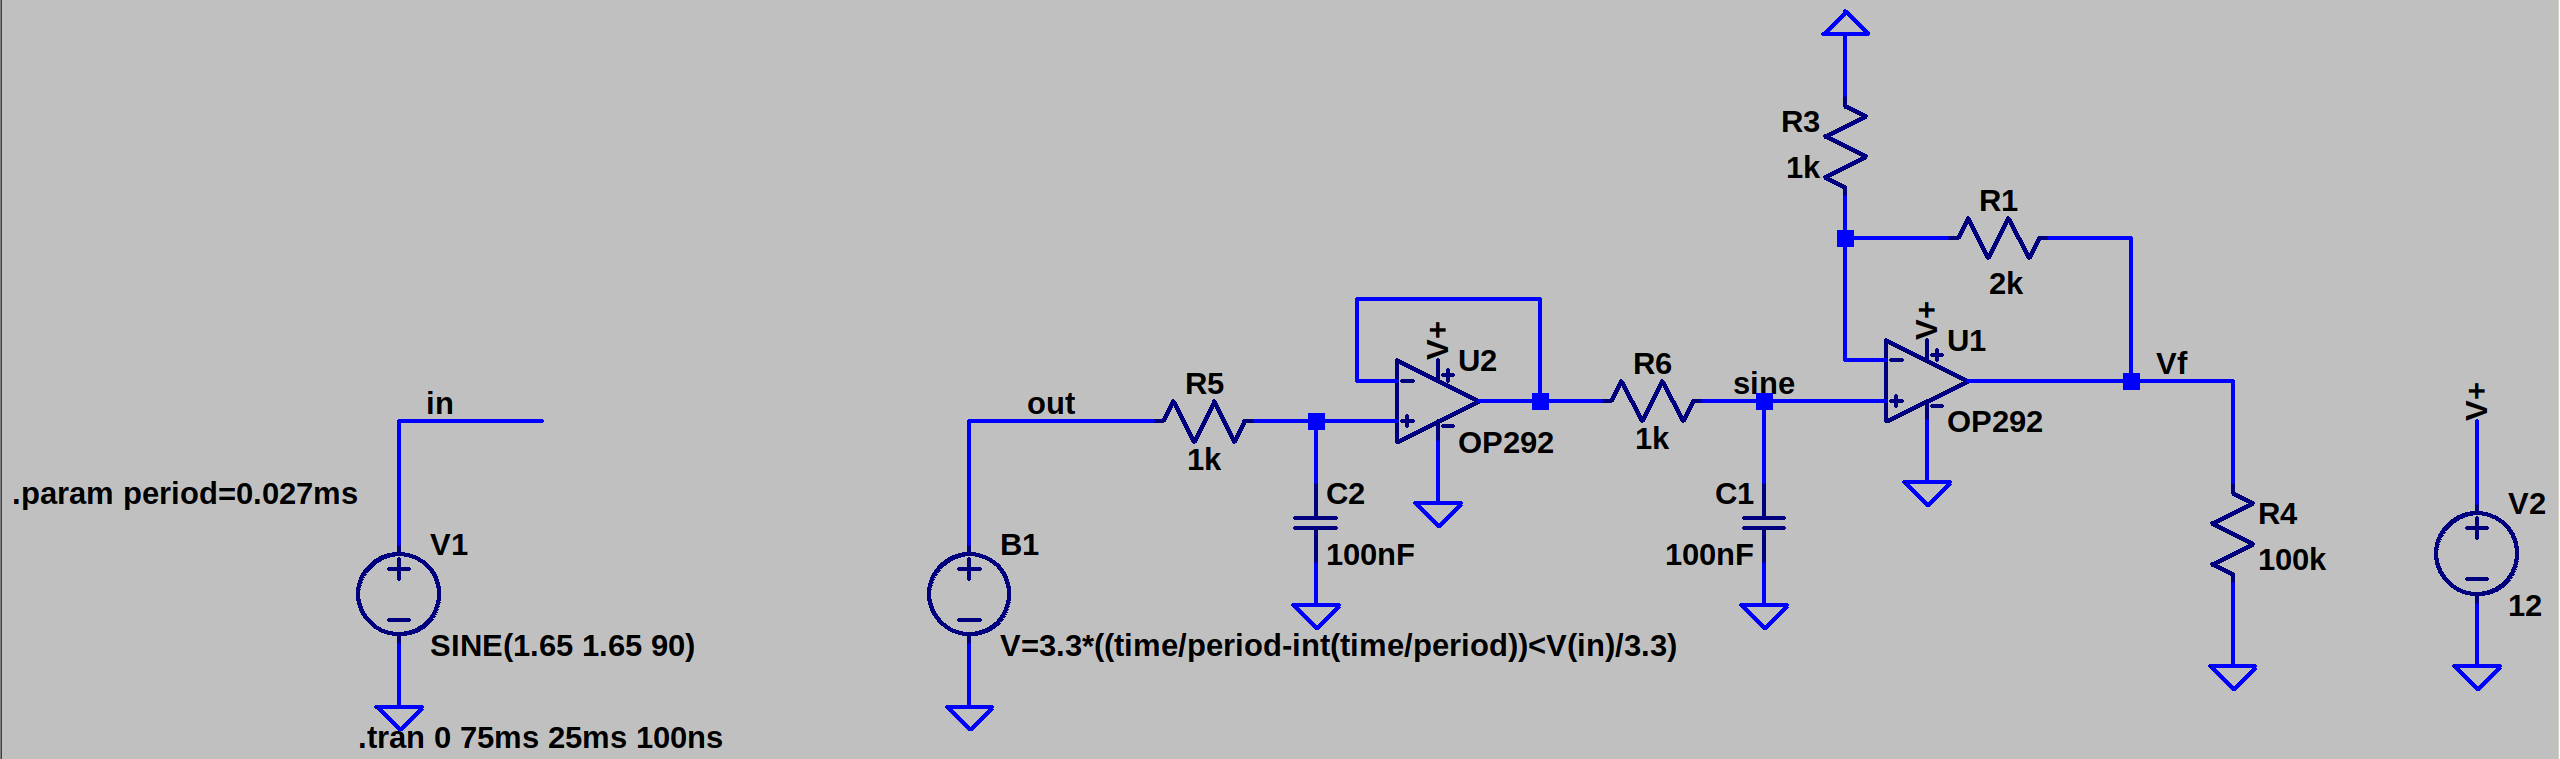
\includegraphics[width=8cm]{./figures/circuit.png}
\caption{The signal generator circuit in LTSpice} 
\label{fig:real_sig_gen}
\end{figure}

The simulation for the architecture in Section~\ref{ssec:second} generates the
relevant voltage responses, provided in Figure~\ref{fig:response}. The top plot
shows the PWM signal generated by Teensy modulating a sine-wave at
$90$\unit{\hertz} frequency. The individual plots in the middle show the output
of the first (cyan) and the second (purple) RC low-pass filters ($v_m$ and
$v_i$, respectivel) that extract the modulated signal from its PWM
representation. Finally, the last plot shows the thrice amplified signal through
the op-amp \texttt{OP292}.

\begin{figure}[t]
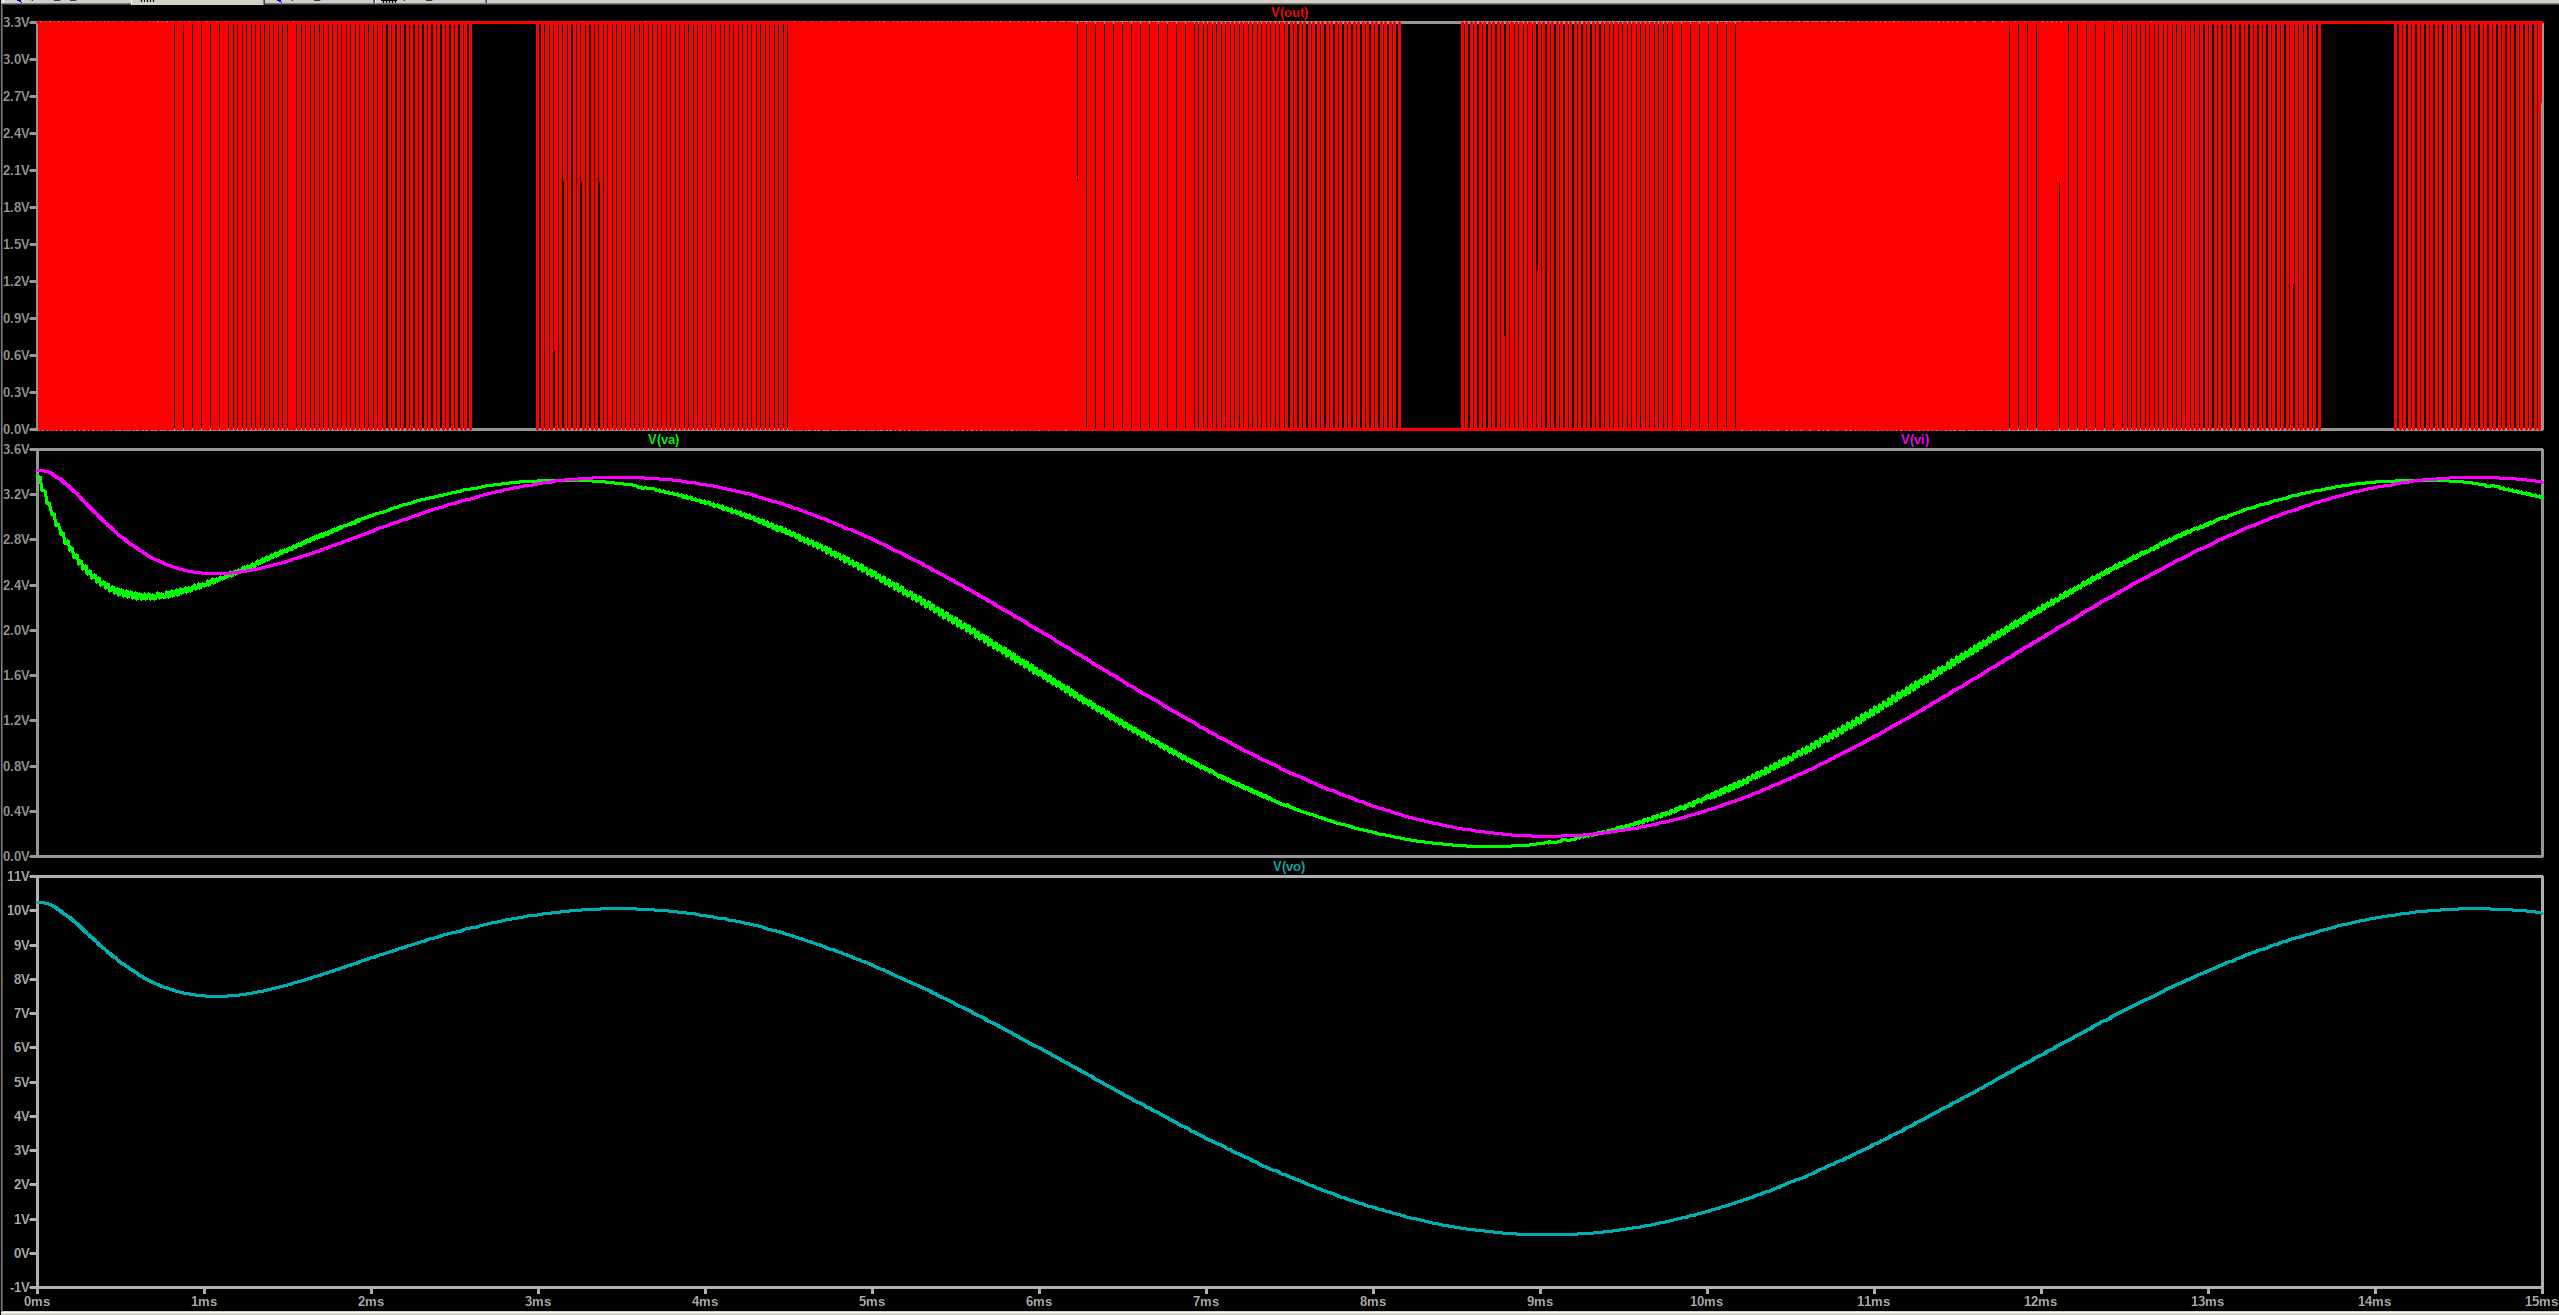
\includegraphics[width=0.5\textwidth]{./figures/pwm_filtered_one_two_final_signal.png}
\caption{The response from the simulation for one full period.} 
\label{fig:response}
\end{figure}


The performance of the Sallen-Key architecture from Section~\ref{ssec:sallenkey}
is shown in Figure~\ref{fig:sallenkey_sim} (top plot), where the values for the
resistances were taken to be $R_1 = R_2 = R = 68$\unit{\kilo\ohm}, $R_f
= 2R_{in} = 1$\unit{\kilo\ohm} and capacitances to be $C_1 = C_2 = C =
1$\unit{\nano\farad}. Even though the performance of the Sallen-Key filter of
Section~\ref{ssec:sallenkey} looks very similar to the $RC$+buffer filter of
Secton~\ref{ssec:second} in simulation, the experiments favor the Sallen-Key
significantly. We will implement this filter in our final design.

\begin{figure}[tbh]
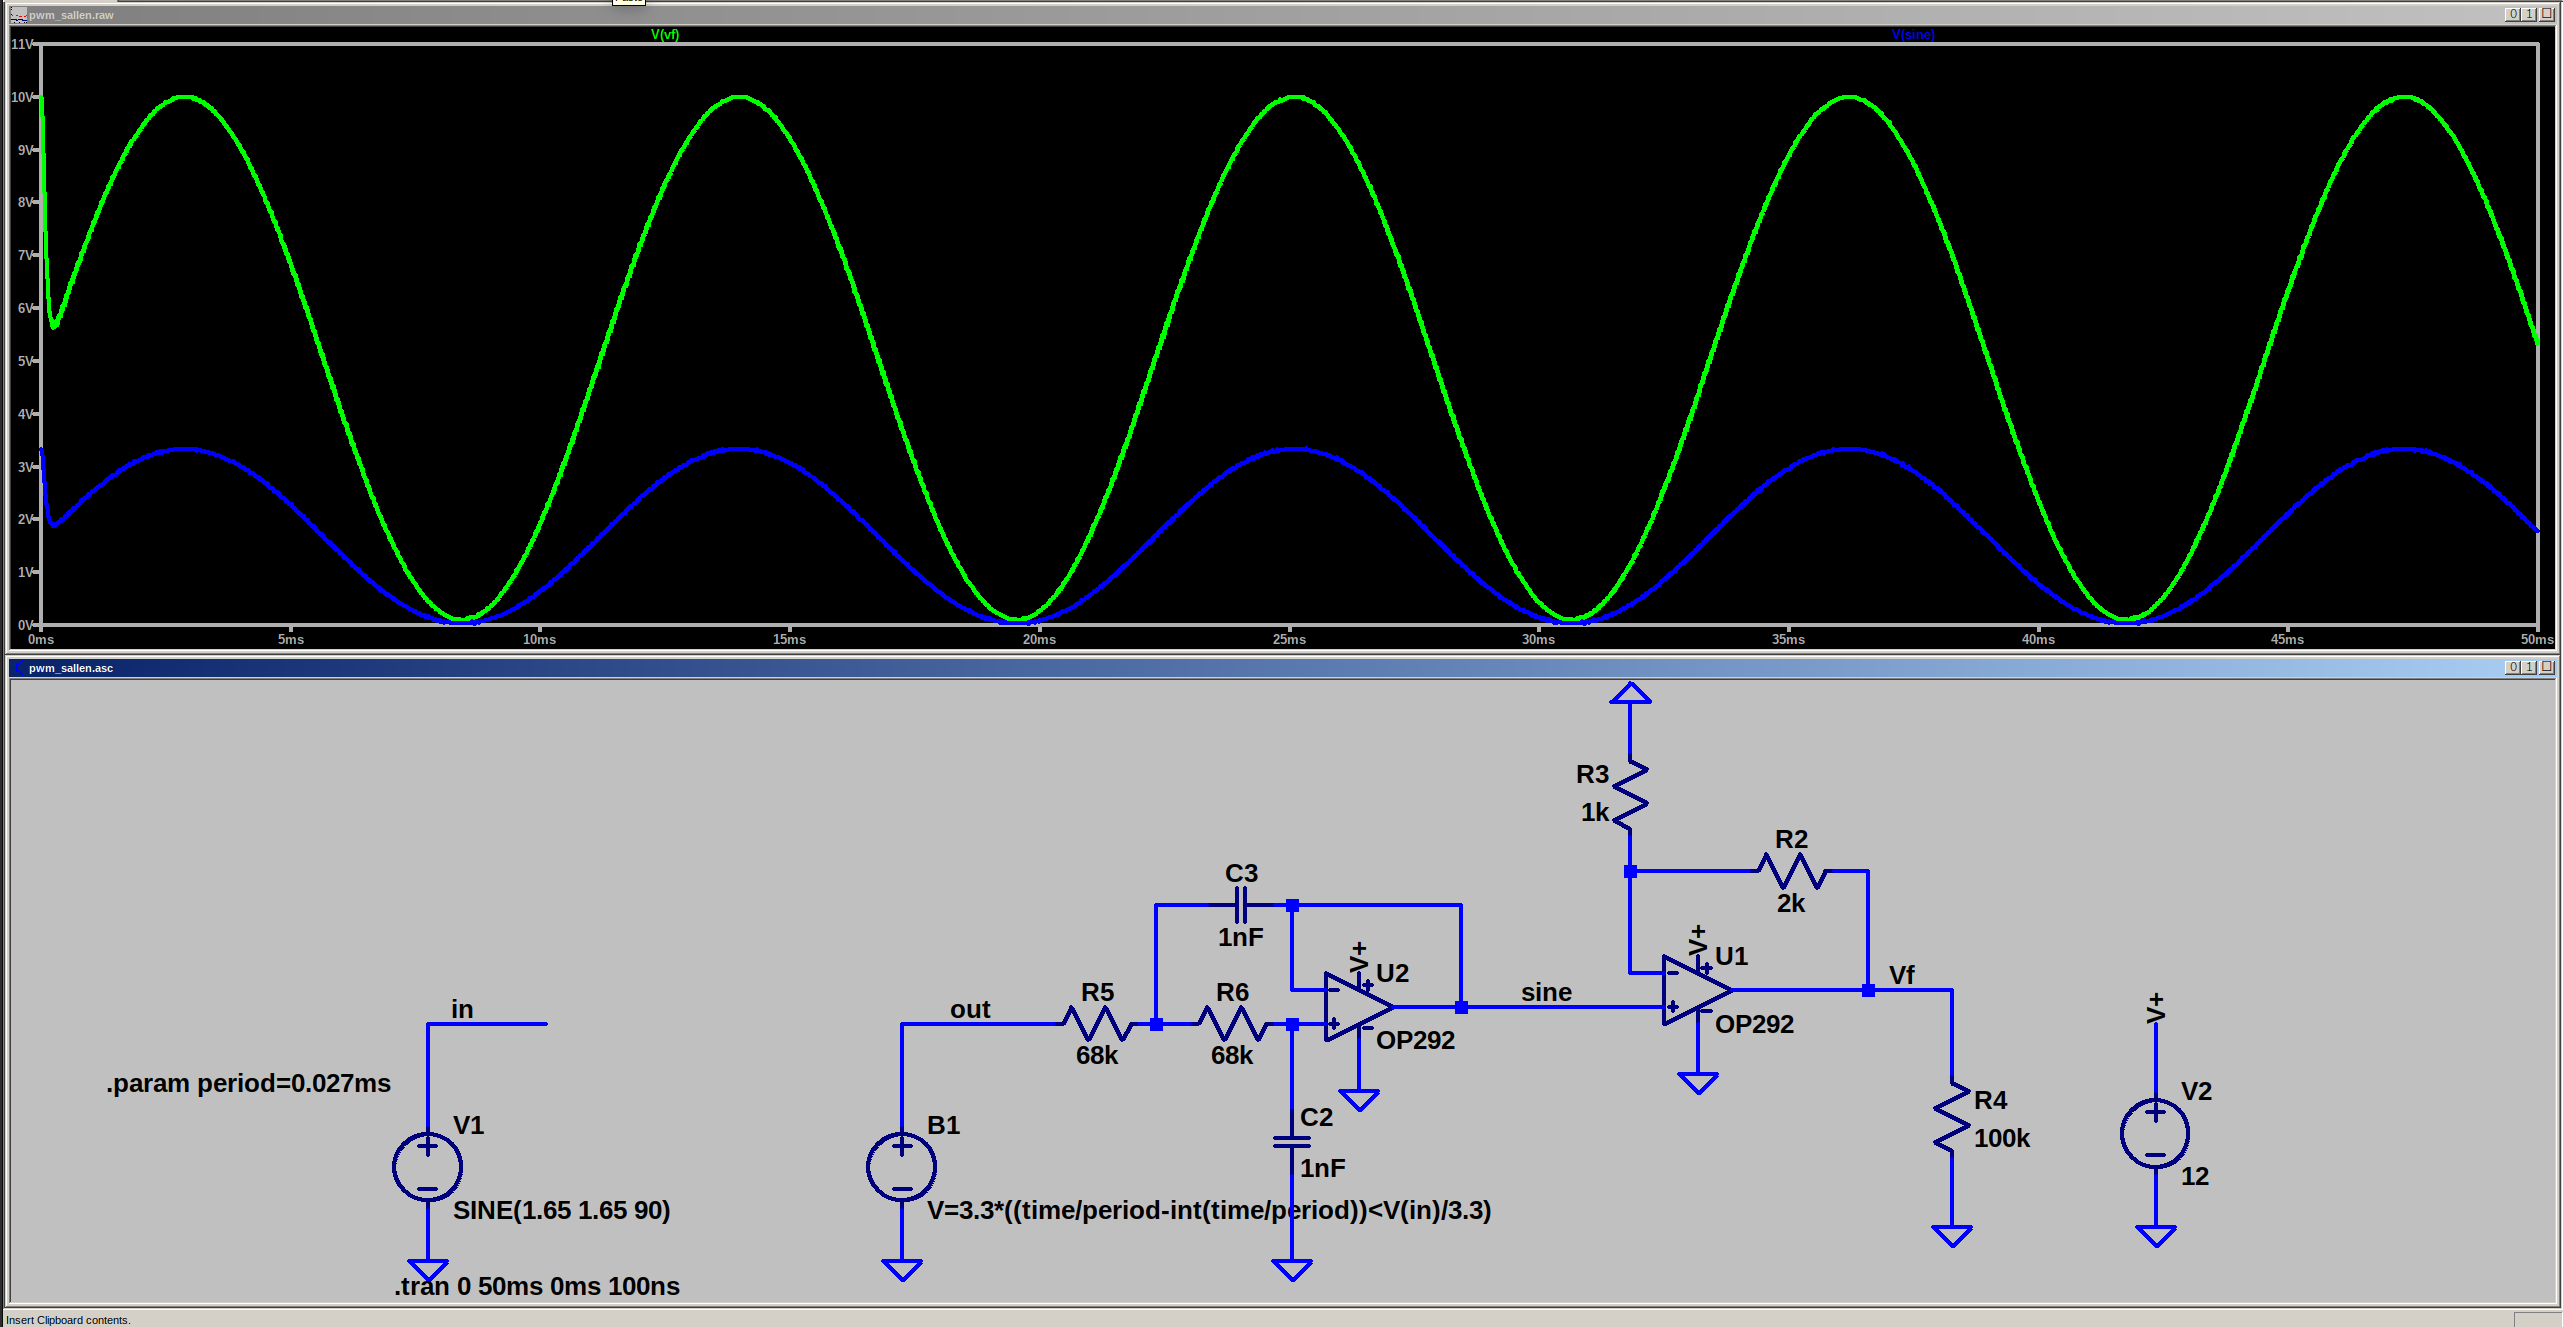
\includegraphics[width=0.5\textwidth]{./figures/sallenkey.png}
\caption{The response of the Sallen-Key architecture.}
\label{fig:sallenkey_sim}
\end{figure}


\vspace{-1em}
\subsection{Experiment}
\vspace{-1em}

The Sallen-Key architecture is implemented on a simple setup on my tabletop.
A snapshot of Teensy's PWM signal that modulates the desired sine-wave output is
provided in Figure~\ref{fig:teensy_pwm}.


\begin{figure}[bh]
    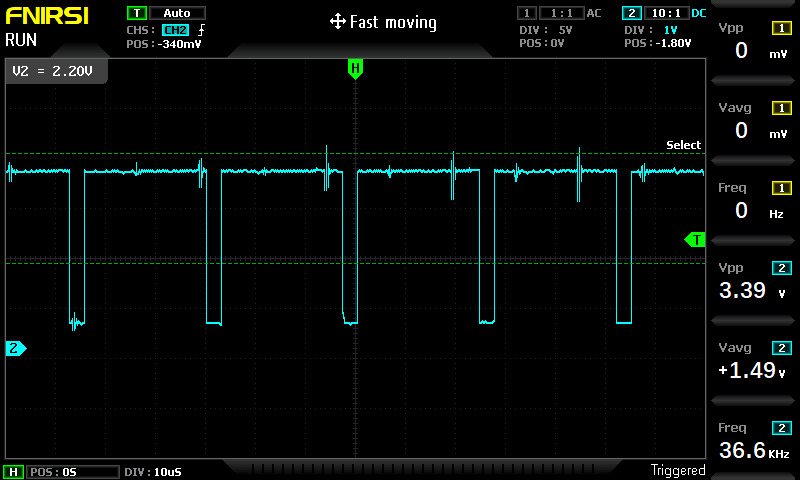
\includegraphics[width=0.5\textwidth]{./figures/teensy_pwm_osc.jpg}
    \caption{A snapshot of Teensy's PWM signal with a carrier frequency of
    $36.6$\unit{\kilo\hertz}.}
    \label{fig:teensy_pwm}
\end{figure}

% \begin{figure}[t]
% 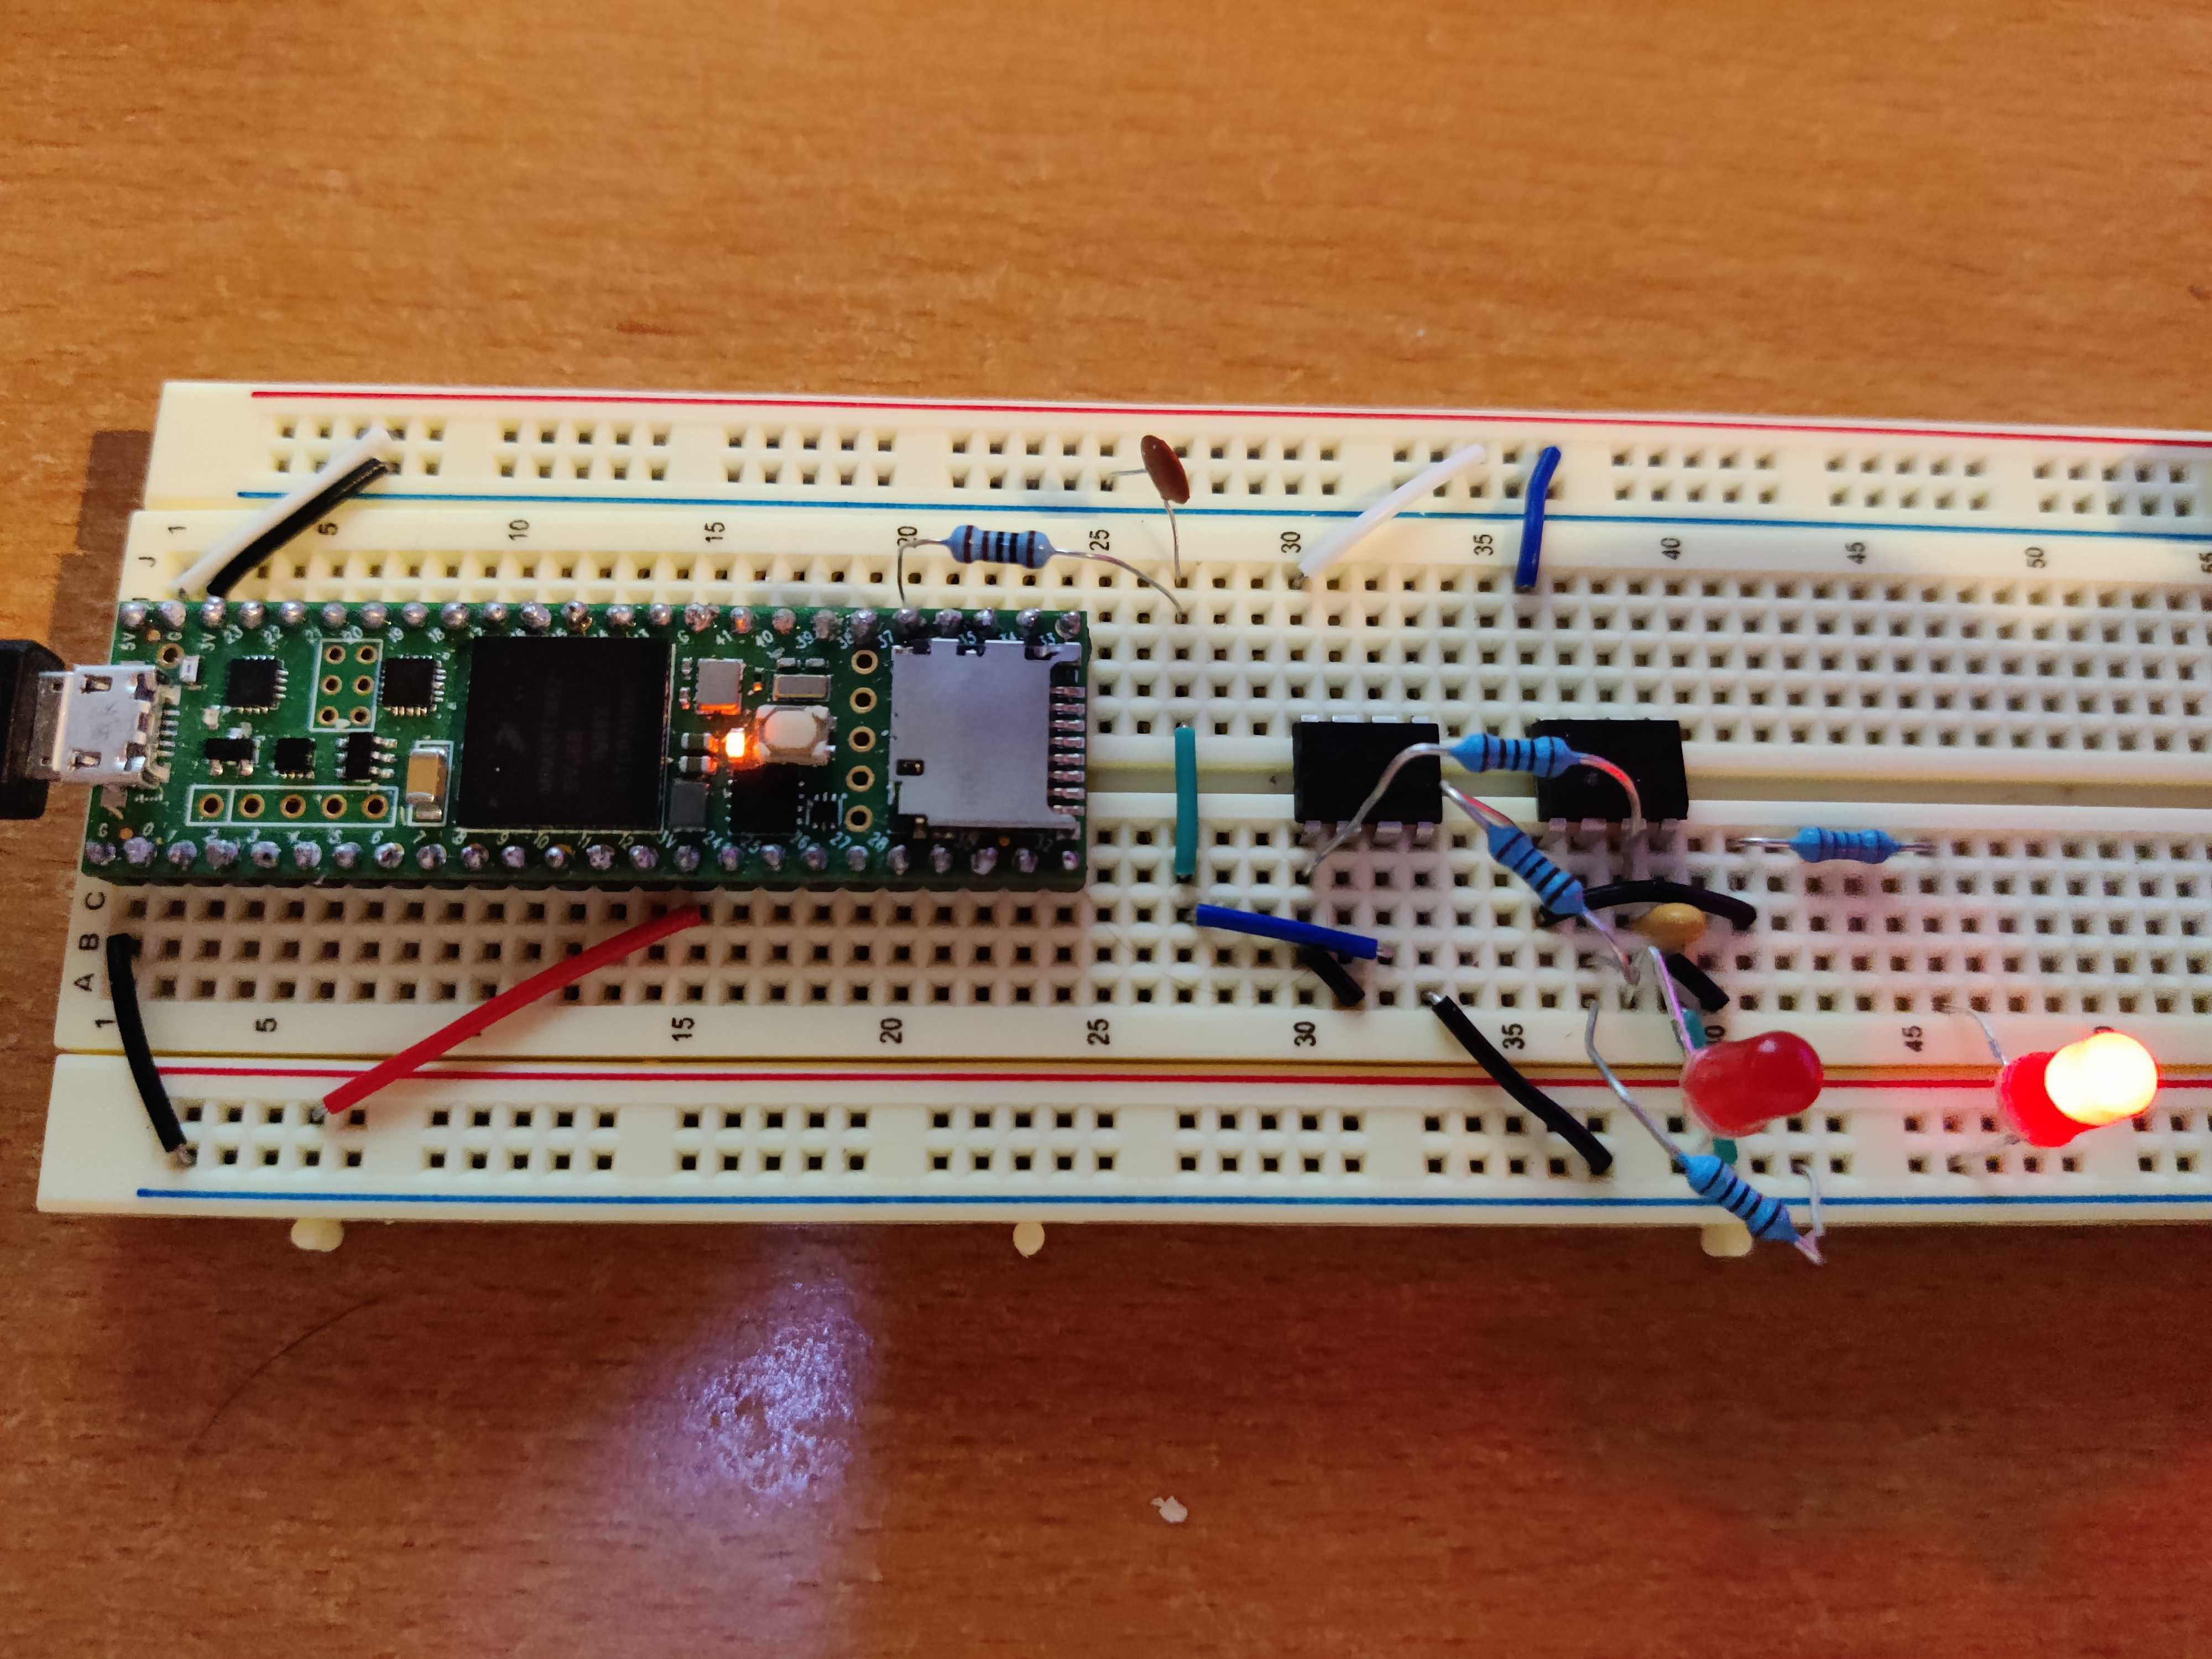
\includegraphics[width=0.5\textwidth]{./figures/prototype.jpg}
% \caption{Prototype working on a LED} 
% \label{fig:exp}
% \end{figure}

Figure~\ref{fig:sallenkey_osc} shows the response of the second-order Sallen-Key
LPF observed through an oscilloscope. This is the output of the signal generator
in response to the Teensy generated $90$\unit{\hertz} $0-3.3$\unit{\volt} PWM
signal modulating the desired sine wave. This response is satisfactory and
should drive the PI controller without any issues.

\begin{figure}[bh]
    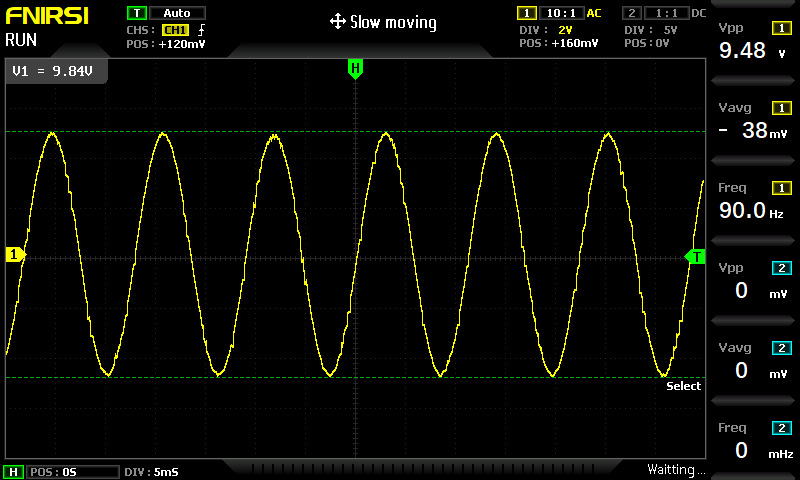
\includegraphics[width=0.5\textwidth]{./figures/output_osc.jpg}
    \caption{The response of the second-order Sallen-Key filter.}
    \label{fig:sallenkey_osc}
\end{figure}

We have also tested the signal generator by driving PI's piezoelectric actuator.
It turns out that since Teensy's imperfect PWM generation, the best values of
the various capacitances and resistances seen in the circuit
diagram~\ref{fig:final_circuit} are as given in Table~\ref{tab:expvalues}. These
are the values to be used in the final design.

{\renewcommand{\arraystretch}{1.5}
\begin{table}
    \centering
    \caption{Experimental values of resistances and capacitances.}
    \begin{tabular}{*6c}
        \toprule
        $R_1$ & $R_2$ & $C_1$ & $C_2$ & $R_f$ & $R_{in}$ \\    
        \hline
        \midrule
        $500$\unit{\kilo\ohm} & $100$\unit{\kilo\ohm} & $2.35$\unit{\nano\farad}
          & $1$\unit{\nano\farad} & $2$\unit{\kilo\ohm} &
        $1$\unit{\kilo\ohm} \\
        \bottomrule
    \end{tabular}
    \label{tab:expvalues}
    \vspace{-1em}
\end{table}
}

\vspace{-1em}
\section{Discussion and Conclusions}
\vspace{-1em}

A sine wave is modulated using a $0-3.3$\unit{\volt} PWM output of a Teensy 4.1
microcontroller at a carrier frequency of $36.6$\unit{\kilo\hertz}. We presented
two second-order lowpass filters to extract the modulated signal from its PWM
representation: (i) $RC$+buffer configuration, (ii) Sallen-Key architecture. We
have shown that in simulation both filters perform similarly, however in
experiments the Sallen-Key filter performs significantly better. We have decided
to use this filter in our final design on the bioreactor.

\section{Acknowledgment}

The first author thanks Drs. John Chiasson and Vishal Saxena of Electrical and
Computer Engineering at Boise State University and Unviersity of Delaware,
respectively, for their invaluable insights into the practical implementation of
the signal generator.


\bibliographystyle{plainnat}
\bibliography{./bib/mechatronics}

%%%%%%%%%%%%%%%%%%%%%%%%%%%%%%%%%%%%%%%%%%%%%%%%%%%%%%%%%%%%%%%%%%%%%%%%%%%%%

\appendix
% \section{Lab Report Policy}
% \begin{enumerate}
% \item Everyone needs to hand in their own lab report. If you work with someone
% in the lab, then put that person's name on the lab report as a collaborator.
% \item Each of you need to collect your own data and write your own report. I do
% not want to see two reports with exactly the same data (even though everyone's
% data will look similar) nor with the same lab report.
% \end{enumerate}
% 
% \section{Typesetting with \LaTeX}
% This document was created using the typesetting language \LaTeX, which allows
% you to create very professional-looking documents with minimal effort. If you
% are interested in learning how to create such documents using \LaTeX, I can
% provide the code that generated this document as a template that you can start
% with.
% 
% %%%%%%%%%%%%%%%%%%%%%%%%%%%%%%%%%%%%%%%%%%%%%%%%%%%%%%%%%%%%%%%%%%%%%%%%%%%%%
% %%%%%%%%%%%%%%%%%%%%%%%%%%%%%%%%%%%%%%%%%%%%%%%%%%%%%%%%%%%%%%%%%%%%%%%%%%%%%
% 
% 
% %%%%%%%%%%%%%%%%%%%%%%%%%%%%%%%%%%%%%%%%%%%%%%%%%%%%%%%%%%%%%%%%%%%%%%%%%%%%%
% 
% % Surround figure environment with turnpage environment for landscape presentation
% \begin{turnpage}
% \begin{figure*}[p]
% 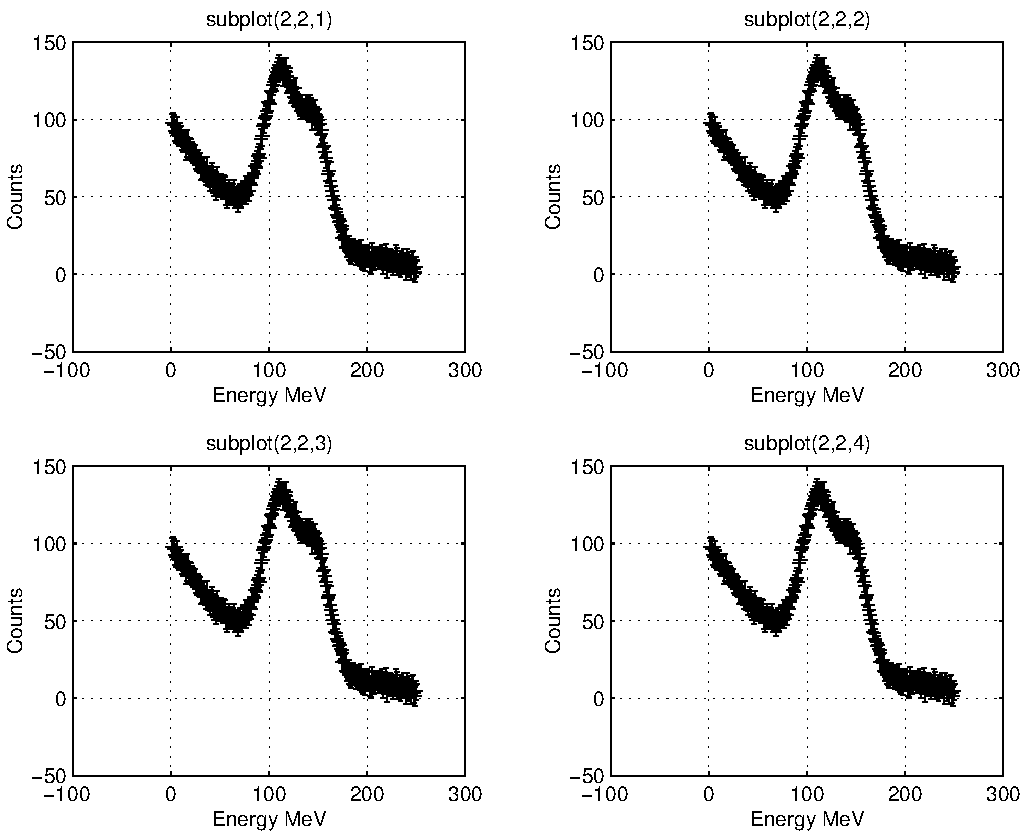
\includegraphics[width=20cm]{./figures/sample-fig5}
% \caption{For very large plots where important detail might be lost
% if too compressed. These full page graphics are usually best kept in
% appendices so as not to impede the flow of the paper.  Note that
% large tables can also be presented in this landscape environment if
% desired.} 
% \label{fig:landscapegraphic}
% \end{figure*}
% \end{turnpage}

% tables should appear as floats within the text
%
% Here is an example of the general form of a table:
% Fill in the caption in the braces of the \caption{} command. Put the label
% that you will use with \ref{} command in the braces of the \label{} command.
% Insert the column specifiers (l, r, c, d, etc.) in the empty braces of the
% \begin{tabular}{} command.
% The ruledtabular enviroment adds doubled rules to table and sets a
% reasonable default table settings.
% Use the table* environment to get a full-width table in two-column
% Add \usepackage{longtable} and the longtable (or longtable*}
% environment for nicely formatted long tables. Or use the the [H]
% placement option to break a long table (with less control than
% in longtable).
% \begin{table}%[H] add [H] placement to break table across pages
% \caption{\label{}}
% \begin{ruledtabular}
% \begin{tabular}{}
% Lines of table here ending with \\
% \end{tabular}
% \end{ruledtabular}
% \end{table}

% To convert program (e.g., C++ Fortran, Matlab, LaTeX\) listings to a
% form easily includable in a \LaTeX\ document
%
% type lgrind -s to see options
% lgrind -llatex -i sample-paper.tex > sampleinputtex
% creates a file sampleinput.tex which can then be included into this
% document simply by uncommenting the next line
%\lgrindfile{testinput.tex}

\vspace{-1em}
\section{Full Circuit Drawing of the Final Design}
\label{sec:fulldesign}
\vspace{-1em}

The final signal generator circuit schematic is presented in
Figure~\ref{fig:final_circuit}. The potential $v_t$ denotes the
$0-3.3$\unit{\volt} PWM signal modulating a $90$\unit{\hertz} sinusoidal wave at
a carrier frequency of $36.6$\unit{\kilo\hertz}. The potential $v_o$ denotes the
$0-10$\unit{\volt} analog $90$\unit{\hertz} sine-wave signal ready to be sent to
the Physik Instrumente controller E-610, depicted in the figure as the impedance
$R_{\text{load}}$, as its reference input. The capacitances and the resistances
are provided in Table~\ref{tab:expvalues}.

\begin{figure*}[b]
\begin{circuitikz}[scale=2, node distance=0.1mm and 0.1mm, rotate=-90, transform
    shape]
\draw (5,.5) node [op amp] (opamp) {\texttt{LM358}}
(opamp.down) -- ++(0,-0.25) node[ground] {}
(0,0) node [left] {$v_t$} to [R, l=$R_1$, o-*] (2,0) node[below]{$v_m$} 
to [R, l=$R_2$, *-*] (opamp.+)
to [C, l_=$C_2$, *-] ($(opamp.+)+(0,-2)$) node [ground] {}
(opamp.out) |- (3.5,2) to [C, l_=$C_1$, *-] (2,2) to [short] (2,0)
(opamp.-) -| (3.5,2)
% (opamp.out) to [short, *-*] (6.5,.5) node (vi) [above] {$v_i$};
(opamp.out) node (vi) [above right = of opamp.out]{$v_i$};
\draw[-latex] (opamp.up) -- ++(0,0.5) node [above] {$V_+$};

\draw (opamp.out) to[short, *-] ++(0.5,0) node[op amp, noinv input up, anchor=+]
(opamp2) {\texttt{LM358}}
(opamp2.-) -- ++(0, -2.0) coordinate (tmp) to [R, l=$R_{in}$, *-] ++(0,-2) node
[ground] (gnd) {} (tmp) to [R, l=$R_f$, -*] (tmp -| opamp2.out) -- (opamp2.out)
to [short, *-o] ++(1,0) node[above]{$v_o$};

\draw let 
    \p1 = (tmp), 
    \p2 = (opamp2.out)
    in
    (\x2, \y1) to [R, l=$R_{\text{load}}$] ++(0, -2) node[ground] {};

\draw (opamp2.down) -- ++(0,-0.25) node[ground] {};
\draw[-latex] (opamp2.up) -- ++(0,0.5) node [above] {$V_+$};

\end{circuitikz}
\caption{The final signal generator circuit design.}
\label{fig:final_circuit}
\end{figure*}



\vspace{-1em}
\section{Alternative Filter}
\vspace{-1em}

During testing, I have mistakenly implemented the circuit presented in
Figure~\ref{fig:alt_circuit}. Later, I analyzed the circuit by figuring out its
transfer function. I include this circuit in here just as an academic curiosity.
It has no bearing on the ISS mission and should be ignored for that purpose.


\begin{figure*}[h]
\begin{circuitikz}[scale=1.5, node distance=0.1mm and 0.1mm, transform shape]
\draw (5,.5) node [op amp] (opamp) {\texttt{LM358}}
(opamp.down) -- ++(0,-0.25) node[ground] {}
(-1,0) node [left] {$v_t$} to [R, l=$R_1$, o-*] (1,0) node[below]{$v_m$} -- ++(0, 0)
to [R, l=$R_2$, -*] (opamp.+)
to [C, l_=$C_2$, *-] ($(opamp.+)+(0,-2)$) node [ground] {}
(opamp.out) |- (3.5,2) to [C, l_=$C_1$, *-, v^=$v_1$] (1,2) to [R, l=$R$] (1,0)
(opamp.-) -| (3.5,2)
% (opamp.out) to [short, *-*] (6.5,.5) node (vi) [above] {$v_i$};
(opamp.out) node (vi) [above right = of opamp.out]{$v_i$};
\draw[-latex] (opamp.up) -- ++(0,0.5) node [above] {$V_+$};

\draw (opamp.out) to[short, *-] ++(0.5,0) node[op amp, noinv input up, anchor=+]
(opamp2) {\texttt{LM358}}
(opamp2.-) -- ++(0, -2.0) coordinate (tmp) to [R, l=$R_{in}$, *-] ++(0,-2) node
[ground] (gnd) {} (tmp) to [R, l=$R_f$, -] (tmp -| opamp2.out) -- (opamp2.out)
to [short, *-o] ++(1,0) node[above]{$v_o$};

% \draw let 
%     \p1 = (tmp), 
%     \p2 = (opamp2.out)
%     in
%     (\x2, \y1) to [R, l=$R_{\text{load}}$] ++(0, -2) node[ground] {};

\draw (opamp2.down) -- ++(0,-0.25) node[ground] {};
\draw[-latex] (opamp2.up) -- ++(0,0.5) node [above] {$V_+$};

\end{circuitikz}
\caption{Alternative LPF circuit.}
\label{fig:alt_circuit}
\end{figure*}


\vspace{-1em}
\subsection{Deriving the equations of the circuit}
\vspace{-1em}

The voltage divider at the inverting input of the second op-amp gives 
%
\begin{equation}
    v_o = \left(1+\nicefrac{R_f}{R_{in}}\right)v_i =: kv_i.
    \label{eq:b1}
\end{equation}
%
Let $i_1$ and $i_2$ be the currents that flow over $C_1$ and $C_2$,
respectively. KVL around various loops give the following relationships
%
\begin{align}
    \label{eq:b2} v_m &= R_2i_2 + v_i, \quad &(v_m - v_i - \text{gnd}),  \\
    \label{eq:b3} v_m &= Ri_1 + v_1 + v_i, \quad &(v_m - v_1 - v_i - \text{gnd}), \\
    \label{eq:b4} v_t &= R_1(i_1 + i_2) + v_m, \quad &(v_t - v_m - \text{gnd}).
\end{align}
% 
The constitutive equations for capacitors provide the last two relevant
equations \[ i_1 = C_1 \dot{v}_1, \qquad i_2 = C_2 \dot{v}_i. \] We want to
obtain an input-output relationship between $v_t$ and $v_o$.

\paragraph{Step 1.} Use constitutive equations for the capacitors to reduce
equations~(\ref{eq:b2}-\ref{eq:b4}).
%
\begin{align*}
    v_m &= R_2C_2\dot{v}_i + v_i = RC_1\dot{v}_1 + v_1 + v_i, \\
    v_t &= R_1C_1\dot{v}_1 + R_1C_2\dot{v}_i + v_m.
\end{align*}

\paragraph{Step 2.} Substitute equation~\eqref{eq:b2} into
equation~\eqref{eq:b4}.
\begin{align*} 
    v_t &= R_1C_1\dot{v}_1 + R_1C_2\dot{v}_i + R_2C_2\dot{v}_i + v_i \\ 
        &= R_1C_1\dot{v}_1 + (R_1+R_2)C_2\dot{v}_i + v_i.
\end{align*}

\paragraph{Step 3.} Eliminate $v_1$ and $\dot{v}_1$.
%
\begin{align*}
    RC_1\dot{v}_t + v_t &= R_1C_1\left(RC_1\ddot{v}_1 + \dot{v}_1 \right) + (R_1
    + R_2)RC_1C_2\ddot{v}_i + \\ 
    &\hspace{2em}RC_1\dot{v}_i + (R_1+R_2)C_2\dot{v}_i + v_i \\
    &= R_1R_2C_1C_2\ddot{v}_i + (R_1+R_2)RC_1C_2\ddot{v}_i + \\
    &\hspace{2em}\left(RC_1 + (R_1+R_2)C_2\right)\dot{v}_i + v_i \\
    &= \underbrace{\left(R_1R_2 + R_1R + R_2R\right)C_1C_2}_{a}\ddot{v}_i + \\
    &\hspace{2em}\underbrace{\left(RC_1 + (R_1+R_2)C_2\right)}_{b}\dot{v}_i + v_i.
\end{align*}
%
where in the second equality, we used the first equations from \textit{Step 1}.
Combining this with equation~\eqref{eq:b1} we obtain the final relationship.
%
\begin{equation}
a\ddot{v}_o + b\dot{v}_o + v_o = k(RC_1\dot{v}_t + v_t).
\label{eq:alt_de}
\end{equation}
%
As a transfer function, we have 
%
\begin{equation}
T(s) = \frac{V_o(s)}{V_t(s)} = k\frac{RC_1s + 1}{as^2 + bs + 1}.
\label{eq:alt_tf}
\end{equation}
%
Note that if $R = 0$, we recover the original Sallen-Key low-pass filter
transfer function~\eqref{eq:tf_sallenkey}:
%
\[\frac{V_o(s)}{V_t(s)} = \frac{k}{R_1R_2C_1C_2s^2 + (R_1+R_2)C_2s + 1}. \]

\vspace{-1em}
\subsection{Analyzing the circuit}
\vspace{-1em}

This filter has a zero in the left-half plane at $z = -\nicefrac{1}{RC_1}$,
in contrast to the original Sallen-Key filter. The presence of the resistance
$R$ is almost always parasitic and does not help with the desired signal
generation.




\end{document}
